\documentclass[12pt, a4paper]{report}
\usepackage[pdftex]{graphicx} %for embedding images
\graphicspath{ {./img/} } %the path to the images
\usepackage[,italian, english]{babel}
\usepackage{url} %for proper url entries
% \usepackage[bookmarks, colorlinks=false, pdfborder={0 0 0}, pdftitle={<pdf title here>}, pdfauthor={<author's name here>}, pdfsubject={<subject here>}, pdfkeywords={<keywords here>}]{hyperref} %for creating links in the pdf version and other additional pdf attributes, no effect on the printed document
%\usepackage[final]{pdfpages} %for embedding another pdf, remove if not required

\begin{document}
\renewcommand\bibname{References} %Renames "Bibliography" to "References" on ref page


\begin{titlepage}

\begin{center}

\Large \textbf {Programmazione Concorrente e Distribuita - Assigment 03 - Part 2B}\\%\\[0.5in]
\vspace{1em}%
\vfill
Leonardo Randacio


Filippo Gurioli


Andrea Biagini
\vspace{1em}
\vfill
{\bf Università di Bologna \\ Scienze e Ingegneria Informatiche}\\[0.5in]

       
\vfill
\today

\end{center}

\end{titlepage}


\tableofcontents
\listoffigures

\newpage
\pagenumbering{arabic} %reset numbering to normal for the main content

\chapter{Analysis}
The goal is to create a collaborative version of the Sudoku game using the 
 built-in Java library "Java RMI". This library provides the functionality 
 of creating two separate JVMs that commuincate, sharing objects and using them as
 if they were locally stored.

A player can create a sudoku grid (a "grid"), view a list of all the
 available grids, join an available grid and collaborate to its completion
 by adding and removing numbers. Every player can also see where the other
 players have the cursor, to have an idea of what they are doing.

\chapter{Design}
The design has been made keeping in mind that the user has to be kept updated
 reactively of the state of the game and the list of the available grids.

\section{Architecture}
The system has a client-server architecture, where the server has all the
 information and the client can obtain a reference of the object it is
 interested in by asking the server.

\section{Visual Formalisms}
\begin{figure}
    \centering
    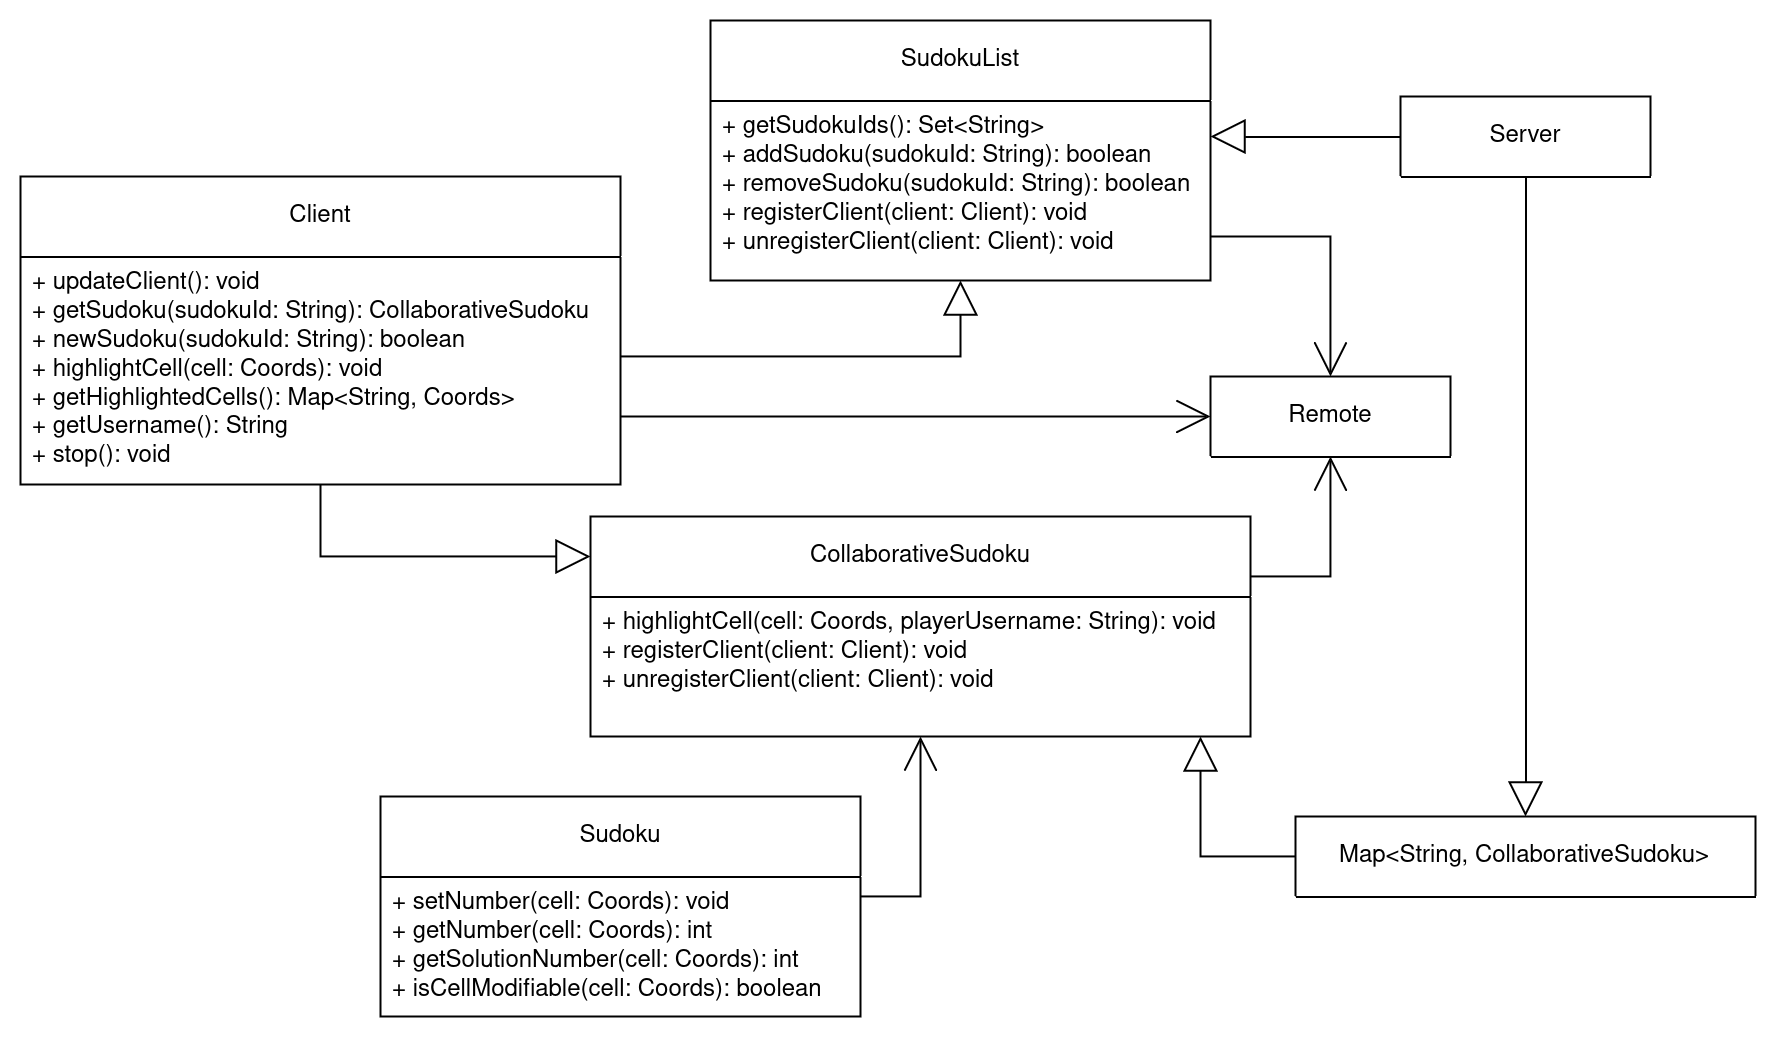
\includegraphics[scale=0.25]{class-diagram.png}
    \caption{UML diagram showing relationships between system components}
\end{figure}

\chapter{Implementation}
Both server and client are implemented in Java, to be able to use the Java RMI
 library. The server part has a model and a tiny controller.

During it's functioning the server prints info messages to the terminal.
 
The client is also composed by a model component (that is remote)
 handled by a controller and a Java Swing GUI to interact with grids.

\section{Problems Encountered}
Relevant implementation details emerge from the problems encountered during the
 development.

\subsection{What objects to share, when to share them}
One of the first problems was detected upon deciding how to structure the model
 component. Sharing all the model in a single object would have been unnecessary
 and not secure, making the system heavier in terms of communication between
 components, and making possible for a client to edit a grid that it is not
 subscribed to.

The solution was to identify every grid with a unique ID (a String has been
 used) and have an object shared by default to every client, containing a set
 of every available grids; in this way, the clients obtain every available ID. The
 action of subscribing to a certain grid corresponds to the client querying a
 remote object referencing the desired grid, and deleting the reference of the
 previously subscribed grid.

\subsection{Remote updates}
In the first implementation of the system remote updates where manually
 requested by the users. This did not satisfy the requirement of a coherently
 updated GUI.

Two solutions have been considered:
The first approach consisted in a separate thread polling the server to obtain 
 updated information. This approach was not efficient and resulted in
 synchronization issues and missed inputs, so it was abandoned. The second
 approach was to use the observer pattern to notify interested clients that an
 update had been made on the server. This approach slightly brakes the RMI
 pattern (in fact, it has been not trivial to implement) but it is a far more
 elegant way to satisfy the requirements as inputs can't be missed and clients
 receive temporarily ordered updates only in what they are interested in, as in
 only the IDs list and the grid they are subscribed to.

\section{Source code organization and execution}
The project is physically divided in a server package and a client package, but
 the model package is shared between both components.

The project is managed by Gradle: use the task "runServer" to run the server
 component and the task "runClient" to run a client. The runClient task takes
 as arguments the username of the player.

\chapter{Conclusions}
In this state, the system is at a good level of development: some improvements
 can be implemented in the GUI, especially from the graphical point of view and
 in the username choice in the client: in the current version of the system it
 has been supposed for simplicity that usernames are unique. This last feature
 can be implemented using a shared object containing all usernames of the
 clients that are currently conneceted.

The Java RMI library is well structured and easy to use once understood its
 basic objects. The downside of this approach, considering this particular
 project, is that Java RMI forces the system to be client-server, where all the
 information and data are stored in the server, making it critical to be kept
 alive. In a peer-to-peer system this disadvantage does not exist.

% \bibliographystyle{plain}
% \bibliography{References}

\end{document}